%==============================================================================
%  Prahari — ET AI Hackathon 2026 · Problem Statement 7
%  Submission document.  Compiles with pdflatex (TeX Live) or Overleaf.
%  --------------------------------------------------------------------------
%  EDIT THESE FOUR LINES, THEN COMPILE (run pdflatex twice for the ToC/refs):
%==============================================================================
\newcommand{\TeamName}{Team Prahari}
\newcommand{\TeamMembers}{Add member names here}
\newcommand{\RepoURL}{https://github.com/Exyons/ET-GenAI-Hackathon-2}
\newcommand{\ContactEmail}{as096255@gmail.com}
%==============================================================================

\documentclass[11pt,a4paper]{article}

\usepackage[T1]{fontenc}
\usepackage[utf8]{inputenc}
\usepackage{lmodern}
\usepackage{amsmath}
\usepackage{amssymb}
\usepackage[margin=2.2cm]{geometry}
\usepackage{microtype}
\usepackage{xcolor}
\usepackage{graphicx}
\usepackage{booktabs}
\usepackage{array}
\usepackage{tabularx}
\usepackage{multicol}
\usepackage{enumitem}
\usepackage{titlesec}
\usepackage{fancyhdr}
\usepackage{tcolorbox}
\usepackage{listings}
\usepackage{tikz}
\usetikzlibrary{arrows.meta,positioning,shapes.geometric,calc,backgrounds,fit}
\usepackage[hidelinks]{hyperref}

%------------------------------------------------------------------ palette ---
\definecolor{ink}{HTML}{0D1526}
\definecolor{violet}{HTML}{534AB7}
\definecolor{violetd}{HTML}{3C3489}
\definecolor{green}{HTML}{1D9E75}
\definecolor{greend}{HTML}{0F6E56}
\definecolor{amber}{HTML}{854F0B}
\definecolor{red}{HTML}{E5484D}
\definecolor{haze}{HTML}{5A6B84}
\definecolor{paper}{HTML}{F5F7FB}
\definecolor{line}{HTML}{D5DCE8}
\definecolor{chip}{HTML}{EEF0FA}

\hypersetup{
  colorlinks=true, linkcolor=violetd, urlcolor=greend, citecolor=violetd,
  pdftitle={Prahari — AI-Driven Cyber Resilience},
  pdfauthor={\TeamName}
}

%--------------------------------------------------------------- headings -----
\titleformat{\section}
  {\normalfont\Large\bfseries\color{violetd}}{\thesection}{0.6em}{}
\titleformat{\subsection}
  {\normalfont\large\bfseries\color{ink}}{\thesubsection}{0.6em}{}
\titlespacing*{\section}{0pt}{1.4em}{0.6em}

\renewcommand{\headrulewidth}{0.4pt}
\pagestyle{fancy}
\fancyhf{}
\fancyhead[L]{\small\color{haze}Prahari · \emph{prahari} — sentinel}
\fancyhead[R]{\small\color{haze}ET AI Hackathon 2026 · PS7}
\fancyfoot[C]{\small\color{haze}\thepage}

%------------------------------------------------------------------ tables ----
\renewcommand{\arraystretch}{1.28}
\newcolumntype{L}[1]{>{\raggedright\arraybackslash}p{#1}}
\newcolumntype{Y}{>{\raggedright\arraybackslash}X}

%------------------------------------------------------------------ boxes -----
\newtcolorbox{keybox}[1][]{
  colback=chip, colframe=violet, boxrule=0.8pt, arc=3pt,
  left=10pt,right=10pt,top=8pt,bottom=8pt, #1}
\newtcolorbox{goldbox}[1][]{
  colback=green!7, colframe=greend, boxrule=0.8pt, arc=3pt,
  left=10pt,right=10pt,top=8pt,bottom=8pt, #1}
\newtcolorbox{warnbox}[1][]{
  colback=amber!8, colframe=amber, boxrule=0.8pt, arc=3pt,
  left=10pt,right=10pt,top=8pt,bottom=8pt, #1}

%------------------------------------------------------------------ code ------
\lstdefinestyle{sh}{
  basicstyle=\ttfamily\footnotesize\color{ink},
  backgroundcolor=\color{paper}, frame=single, rulecolor=\color{line},
  breaklines=true, showstringspaces=false, columns=fullflexible,
  keepspaces=true, xleftmargin=6pt, xrightmargin=2pt, aboveskip=6pt, belowskip=6pt}
\lstset{style=sh}

% pill / chip macro
\newcommand{\pill}[2]{\tikz[baseline=-0.55ex]\node[fill=#1,text=white,rounded corners=3pt,inner sep=2pt,font=\scriptsize\bfseries]{#2};}

\begin{document}

%============================================================== TITLE PAGE =====
\begin{titlepage}
\thispagestyle{empty}
\begin{tikzpicture}[remember picture,overlay]
  \fill[ink] (current page.north west) rectangle ([yshift=-6cm]current page.north east);
  \node[anchor=north west, text=paper, font=\Huge\bfseries]
        at ([xshift=2.2cm,yshift=-2.0cm]current page.north west) {PRAHARI};
  \node[anchor=north west, text=green!80!white, font=\large]
        at ([xshift=2.25cm,yshift=-3.3cm]current page.north west)
        {\textit{prahari} \; ·  \; ``the sentinel that watches the perimeter''};
  \node[anchor=north west, text=paper!70, font=\normalsize]
        at ([xshift=2.25cm,yshift=-4.2cm]current page.north west)
        {AI-Driven Cyber Resilience for Critical National Infrastructure};
\end{tikzpicture}

\vspace{7.5cm}

{\Large\bfseries\color{ink} Behavioural threat detection that fuses auth, network and
endpoint telemetry into one incident timeline — mapped to MITRE ATT\&CK\ with cited
reasoning, and running fully air-gapped.\par}

\vspace{0.8cm}
\begin{keybox}
\begin{tabularx}{\linewidth}{@{}l Y@{}}
\textbf{Event}        & ET AI Hackathon 2026 \\
\textbf{Problem Statement} & PS7 — Multi-Agent AI for Cyber Resilience of Critical National Infrastructure \\
\textbf{Submission}   & \TeamName \\
\textbf{Team}         & \TeamMembers \\
\textbf{Repository}   & \url{\RepoURL} \\
\textbf{Contact}      & \href{mailto:\ContactEmail}{\ContactEmail} \\
\end{tabularx}
\end{keybox}

\vspace{0.4cm}
\begin{goldbox}
\textbf{One-line thesis.}\; Real machine learning does the \emph{detection}; the local LLM
only \emph{reasons and explains}. Every automated decision traces back to the exact raw log
records that triggered it — and nothing ever leaves the perimeter.
\end{goldbox}

\vfill
{\small\color{haze} Prepared for hackathon evaluation. All benchmark figures in this document
are measured on real LANL red-team data and reproducible from the repository.\par}
\end{titlepage}

%============================================================== CONTENTS =======
\tableofcontents
\thispagestyle{fancy}
\newpage

%============================================================== 1. SUMMARY =====
\section{Executive Summary}

Critical national infrastructure — power grids, water systems, transport, defence networks —
is now attacked by \emph{advanced persistent threats} (APTs) that never trip a signature.
They log in with valid stolen credentials, move laterally between internal hosts, and beacon
out quietly. Each individual event looks legitimate. The attack only becomes visible when you
\emph{correlate across sensors} and read the \emph{behaviour}.

\textbf{Prahari} is a multi-agent Security Operations Center (SOC) that does exactly this. It
ingests authentication, process/endpoint and network telemetry into a single canonical event
schema, learns a behavioural baseline \emph{per entity}, and fuses co-occurring anomalies
across all three sources into one scored incident on one host's timeline. It then maps that
incident to MITRE ATT\&CK\ techniques using a grounded, retrieval-augmented local LLM, predicts
the adversary's likely next tactic, and recommends a containment action behind a human gate.

The entire system runs \textbf{air-gapped} — no cloud API, no data egress — which is the
non-negotiable requirement for classified OT/IT telemetry and the differentiator no
cloud-hosted SOC can match on sovereign infrastructure.

\begin{keybox}
\textbf{Headline result (measured on real LANL red-team logs):} behavioural detection recalls
\textbf{79\%} of genuine red-team lateral movement where the signature/IOC baseline recalls
\textbf{0\%}; cross-source fusion produces \textbf{high-confidence incidents on 9 of 11}
red-team hosts; ATT\&CK\ attribution runs entirely on local models with a hallucination guard.
\end{keybox}

%============================================================== 2. PROBLEM =====
\section{The Problem}

\subsection{Why signatures fail on national infrastructure}

Signature and indicator-of-compromise (IOC) detection asks ``have I seen this exact bad thing
before?'' APT tradecraft is built to defeat that question:

\begin{itemize}[leftmargin=1.4em,itemsep=2pt]
  \item \textbf{Valid credentials.} A stolen-but-legitimate NTLM login to an internal host has
        no malicious signature — it is a normal authentication event.
  \item \textbf{Living off the land.} \texttt{whoami}, \texttt{net use}, PowerShell — native
        tools, no malware to fingerprint.
  \item \textbf{Low and slow.} Steps are spread across sensors and time so no single log looks
        alarming.
\end{itemize}

The intelligence is not in any one event; it is in the \emph{relationship} between an
anomalous login, an unusual process, and an outbound connection on the same host within a
short window. Detecting that requires (a) behavioural baselining rather than rules, and
(b) fusion across otherwise-siloed telemetry.

\subsection{The sovereignty constraint}

For critical national infrastructure the telemetry is classified and \emph{legally cannot
leave the operational perimeter}. That rules out every SOC product built around a cloud LLM
API. A credible solution must deliver the AI reasoning \textbf{locally}.

%============================================================== 3. SOLUTION ====
\section{Solution Overview}

Prahari is organised as a deterministic ingestion spine feeding a set of cooperating agents,
surfaced through a live Next.js SOC console.

\begin{keybox}
\begin{center}
\ttfamily\small
raw logs $\rightarrow$ CanonicalEvent $\rightarrow$ enrich $\rightarrow$ Sentinel (ML anomaly)
$\rightarrow$ Correlator (fuse $\rightarrow$ Incident) \\[2pt]
$\rightarrow$ Attributor (ATT\&CK RAG, local LLM) + Predictor $\rightarrow$ FastAPI $\rightarrow$ Next.js console
\end{center}
\end{keybox}

\subsection{Architecture at a glance}

\begin{center}
\resizebox{\linewidth}{!}{%
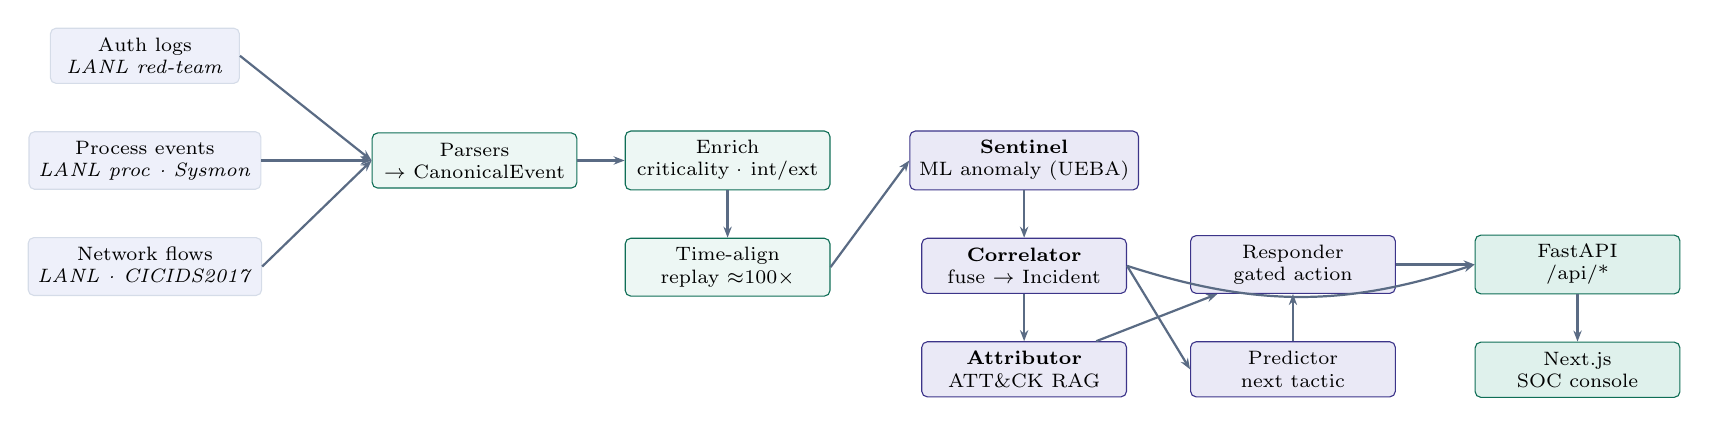
\begin{tikzpicture}[
   font=\scriptsize,
   node distance=6mm,
   src/.style   ={draw=line,fill=chip,rounded corners=2pt,minimum height=7mm,minimum width=24mm,align=center},
   spine/.style ={draw=greend,fill=green!8,rounded corners=2pt,minimum height=7mm,minimum width=26mm,align=center},
   agent/.style ={draw=violetd,fill=violet!12,rounded corners=2pt,minimum height=7mm,minimum width=26mm,align=center},
   outp/.style  ={draw=greend,fill=green!14,rounded corners=2pt,minimum height=7mm,minimum width=26mm,align=center},
   fl/.style    ={-{Stealth[length=4pt]},draw=haze,thick}
  ]
  % sources
  \node[src] (a1) {Auth logs\\\textit{LANL red-team}};
  \node[src,below=of a1] (a2) {Process events\\\textit{LANL proc · Sysmon}};
  \node[src,below=of a2] (a3) {Network flows\\\textit{LANL · CICIDS2017}};

  % spine
  \node[spine,right=14mm of a2] (par) {Parsers\\$\rightarrow$ CanonicalEvent};
  \node[spine,right=6mm of par] (en) {Enrich\\criticality · int/ext};
  \node[spine,below=6mm of en] (rp) {Time-align\\replay $\approx$100$\times$};

  % agents
  \node[agent,right=10mm of en] (sent) {\textbf{Sentinel}\\ML anomaly (UEBA)};
  \node[agent,below=6mm of sent] (cor) {\textbf{Correlator}\\fuse $\rightarrow$ Incident};
  \node[agent,below=6mm of cor] (att) {\textbf{Attributor}\\ATT\&CK RAG};
  \node[agent,right=8mm of att] (pred) {Predictor\\next tactic};
  \node[agent,above=6mm of pred] (resp) {Responder\\gated action};

  % outputs
  \node[outp,right=10mm of resp] (api) {FastAPI\\/api/*};
  \node[outp,below=6mm of api] (ui) {Next.js\\SOC console};

  \draw[fl] (a1.east) -- (par.west);
  \draw[fl] (a2.east) -- (par.west);
  \draw[fl] (a3.east) -- (par.west);
  \draw[fl] (par) -- (en);
  \draw[fl] (en) -- (rp);
  \draw[fl] (rp.east) -- (sent.west);
  \draw[fl] (sent) -- (cor);
  \draw[fl] (cor) -- (att);
  \draw[fl] (cor.east) -- (pred.west);
  \draw[fl] (att) -- (resp);
  \draw[fl] (pred) -- (resp);
  \draw[fl] (resp) -- (api);
  \draw[fl] (cor.east) to[bend right=18] (api.west);
  \draw[fl] (api) -- (ui);
\end{tikzpicture}}
\end{center}

\begin{goldbox}
\textbf{The golden rule.} Everything before the Attributor is deterministic Python +
scikit-learn. The LLM never decides \emph{whether} something is an attack — it only
\emph{names} an attack the ML already found, and only from a retrieved candidate set. This
keeps the system auditable and immune to LLM hallucination in the detection path.
\end{goldbox}

\subsection{Agent topology → problem-statement coverage}

Five agents map onto the five capabilities the problem statement asks for. Three are built in
depth; two are lightweight but functional — full coverage, anchored by depth where it matters.

\begin{center}
\begin{tabularx}{\linewidth}{@{}L{2.4cm} Y L{4.3cm} L{2.6cm}@{}}
\toprule
\textbf{Agent} & \textbf{Job} & \textbf{Brain} & \textbf{PS component} \\
\midrule
\textbf{Sentinel}   & Per-entity behavioural baselines; scores deviations & Isolation Forest + learned novelty (UEBA) & 1 · Behavioural anomaly \\
\textbf{Correlator} & Fuse multi-source events into one Incident & Deterministic kill-chain phases + compound score & Challenge core \\
\textbf{Attributor} & Map Incident to ATT\&CK\ techniques, cited & RAG: \texttt{embeddinggemma} + \texttt{qwen2.5} (local) & 2 · APT attribution \\
\textbf{Predictor}  & Likely next tactic & Markov chain over ATT\&CK\ tactics & 2 · APT prediction \\
\textbf{Responder}  & Gated containment recommendation & Playbook catalogue + human triple-gate & 3 · Autonomous response \\
Vuln view           & CVE / asset criticality context & Lookup / CMDB enrichment & 4 · Vuln prioritisation \\
Digital twin        & Attack-path / lateral view & Graph view (attack map) & 5 · Resilience twin \\
\bottomrule
\end{tabularx}
\end{center}

%============================================================== 4. DETECTION ===
\section{Detection — Behaviour, Not Signatures}

Detection lives in two ML detectors: \textbf{Sentinel} (authentication) and
\textbf{NetworkSentinel} (flows). This is where the ``detect by behaviour'' claim is earned.

\subsection{Per-entity feature engineering (UEBA)}

\texttt{AuthBaseline} learns what is normal \emph{for each user} from history — the hosts they
log into, the hosts they log in \emph{from}, their usual authentication mechanisms, and their
active hours. Each event is then reduced to five interpretable novelty signals in $[0,1]$:

\begin{center}
\begin{tabularx}{\linewidth}{@{}L{3.2cm} Y L{4.4cm}@{}}
\toprule
\textbf{Feature} & \textbf{Meaning} & \textbf{A value of 1.0 means} \\
\midrule
\texttt{is\_new\_dest}      & Host never seen for this user & Lateral move to a new machine \\
\texttt{is\_new\_src}       & Source host never seen        & Logging in from somewhere new \\
\texttt{auth\_type\_rarity} & $1-\text{freq}(\text{auth type})$ & Rare mechanism (NTLM where Kerberos is normal $\approx$ pass-the-hash) \\
\texttt{hour\_novelty}      & Active hour never seen        & A 3\,a.m.\ login \\
\texttt{dest\_criticality}  & Asset importance (0.25–1.0)   & Targeting a critical host \\
\bottomrule
\end{tabularx}
\end{center}

The baseline is \emph{learned from data}, not hand-written rules, and it is
\emph{interpretable}: an alert reads literally as ``new destination + NTLM + off-hours +
critical asset.''

\subsection{Isolation Forest}

Sentinel scores each five-feature vector with an Isolation Forest: an ensemble of random trees
that isolates anomalies in few splits (anomalies are ``few and different'', so they separate
early). The behavioural feature space means novelty — not a known-bad signature — is what
drives the score. NetworkSentinel applies the same idea to flow features after
\texttt{StandardScaler} normalisation.

\subsection{The honest single-source finding}

\begin{warnbox}
Measured on real LANL data, an \emph{auth-only, per-event} novelty threshold recalls
\textbf{79\%} of red-team lines but at brutal precision (0.4\%, $\approx$15k false positives) —
real users constantly touch new hosts and log in at odd hours. We swept thresholds and added a
compound novelty gate: neither fixes single-source precision. \textbf{This is the empirical
justification for the architecture: precision is not a threshold problem, it is a fusion
problem.}
\end{warnbox}

%============================================================== 5. FUSION ======
\section{The Money Moment — Cross-Source Fusion}

The Correlator is the heart of the system. It groups anomalous events by entity within a time
window, tags each with its kill-chain phase, and computes a \emph{compound score}. Three
unremarkable events, fused on one host's timeline, trace an intrusion no single sensor would
flag:

\begin{center}
\begin{tikzpicture}[font=\footnotesize, node distance=3mm,
   ev/.style={draw=line,fill=paper,rounded corners=2pt,minimum height=8mm,text width=6.4cm,align=left,inner sep=5pt}]
  \node[ev] (e1) {\pill{violet}{AUTH} \; \texttt{15:32:16}\; U342 $\rightarrow$ C553 remote login (NTLM) \hfill \color{red}\textbf{[redteam]}};
  \node[ev,below=of e1] (e2) {\pill{amber}{PROCESS} \; \texttt{15:32:19}\; \texttt{cmd /c whoami} on C553};
  \node[ev,below=of e2] (e3) {\pill{green}{NETWORK} \; \texttt{15:32:24}\; C553 $\rightarrow$ 52.84.23.17 outbound beacon};
  \node[draw=violetd,fill=violet!12,rounded corners=3pt,below=5mm of e3,text width=8.2cm,align=center,inner sep=6pt] (c)
       {\textbf{Correlator:} 3 sensors · 3 kill-chain phases · 8 seconds · one host\\
        compound score \textbf{0.94} → \textbf{HIGH-CONFIDENCE incident}\\[2pt]
        \color{haze}\textit{Signature baseline over the same data: silent.}};
  \draw[-{Stealth[length=4pt]},haze,thick] (e1) -- (e2);
  \draw[-{Stealth[length=4pt]},haze,thick] (e2) -- (e3);
  \draw[-{Stealth[length=4pt]},violetd,thick] (e3) -- (c);
\end{tikzpicture}
\end{center}

\begin{goldbox}
\textbf{This is verified on real data, not synthetic.} On the genuine LANL red-team host set,
correlating by target host fused auth + process + network into \textbf{high-confidence
incidents for 9 of 11} red-team hosts — each spanning all three sources and three kill-chain
phases (lateral movement + execution + command-and-control). The ``C553 moment'' exists in the
real capture.
\end{goldbox}

%============================================================== 6. ATTRIBUTION =
\section{ATT\&CK Attribution — Grounded RAG, Air-Gapped}

Once an incident exists, the Attributor names \emph{what} it is in MITRE ATT\&CK\ terms — with
citations, and without ever leaving the box.

\begin{center}
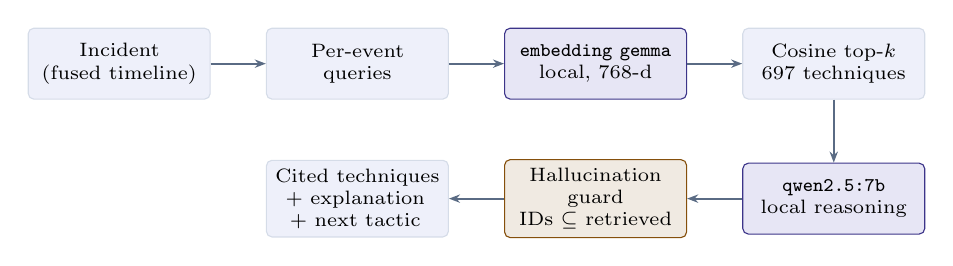
\begin{tikzpicture}[font=\scriptsize, node distance=7mm,
   b/.style={draw=line,fill=chip,rounded corners=2pt,minimum height=9mm,text width=2.1cm,align=center,inner sep=3pt},
   llm/.style={draw=violetd,fill=violet!14,rounded corners=2pt,minimum height=9mm,text width=2.1cm,align=center,inner sep=3pt},
   g/.style={draw=amber,fill=amber!12,rounded corners=2pt,minimum height=9mm,text width=2.1cm,align=center,inner sep=3pt},
   fl/.style={-{Stealth[length=4pt]},draw=haze,thick}]
  \node[b] (inc) {Incident\\(fused timeline)};
  \node[b,right=of inc] (q) {Per-event queries};
  \node[llm,right=of q] (emb) {\texttt{embedding} \texttt{gemma}\\local, 768-d};
  \node[b,right=of emb] (ret) {Cosine top-$k$\\697 techniques};
  \node[llm,below=8mm of ret] (llm) {\texttt{qwen2.5:7b}\\local reasoning};
  \node[g,left=of llm] (guard) {Hallucination guard\\IDs $\subseteq$ retrieved};
  \node[b,left=of guard] (out) {Cited techniques\\+ explanation\\+ next tactic};
  \draw[fl] (inc)--(q); \draw[fl] (q)--(emb); \draw[fl] (emb)--(ret);
  \draw[fl] (ret)--(llm); \draw[fl] (llm)--(guard); \draw[fl] (guard)--(out);
\end{tikzpicture}
\end{center}

\begin{itemize}[leftmargin=1.4em,itemsep=2pt]
  \item \textbf{Retrieval.} Each timeline step is embedded locally with \texttt{embeddinggemma}
        and matched by cosine similarity against 697 MITRE ATT\&CK\ enterprise techniques held
        in memory (numpy) — no external vector database needed for $\approx$700 documents.
  \item \textbf{Reasoning.} \texttt{qwen2.5:7b} maps each step to techniques and writes a cited
        explanation. Querying \emph{per timeline step} (not one incident-level query) is what
        makes lateral-movement and C2 techniques surface instead of being swamped by discovery.
  \item \textbf{Hallucination guard.} Any technique ID the LLM emits must be a member of the
        retrieved candidate set, or it is rejected. The model literally cannot invent a
        technique that was not grounded in retrieval.
\end{itemize}

\subsection{Measured attribution of the C553 incident}

\begin{center}
\begin{tabularx}{\linewidth}{@{}Y L{4.6cm} L{3.0cm}@{}}
\toprule
\textbf{Timeline step} & \textbf{Technique} & \textbf{Correct?} \\
\midrule
NTLM remote login (lateral movement) & \textbf{T1021.006} Remote Services & \checkmark\ family \\
\texttt{cmd /c whoami} (discovery)    & \textbf{T1057} Process Discovery   & \checkmark\ exact \\
Outbound beacon (C2)                  & \textbf{T1071.002} App-Layer Protocol & \checkmark\ family \\
\bottomrule
\end{tabularx}
\end{center}

\noindent\textbf{Predicted next tactic:} \texttt{command-and-control $\rightarrow$ exfiltration (1.0)},
from a Markov model over ATT\&CK\ tactic transitions. All three cited IDs were present in the
retrieved candidate set; no un-retrieved ID could be emitted.

%============================================================== 7. RESPONSE ====
\section{Response — Recommendation Behind a Human Gate}

The Responder proposes containment (e.g.\ \texttt{block\_ip}) from a playbook catalogue that
records each action's \emph{what} and \emph{blast-radius impact}. It is deliberately
conservative:

\begin{itemize}[leftmargin=1.4em,itemsep=2pt]
  \item \textbf{Public-only blocking.} IPs are classified as internal (RFC1918) or public;
        \texttt{block\_ip} is only ever recommended for public destinations, so a response
        never proposes black-holing an internal host.
  \item \textbf{Dry-run by default.} Actions execute in dry-run unless explicitly armed.
  \item \textbf{Triple human gate.} Arm $\rightarrow$ approve $\rightarrow$ execute, each a distinct step,
        with a revert path. Autonomy is bounded by design; a human is always in the loop for
        anything that touches production.
\end{itemize}

%============================================================== 8. DEPLOY ======
\section{Sovereign, Air-Gapped Deployment}

\begin{center}
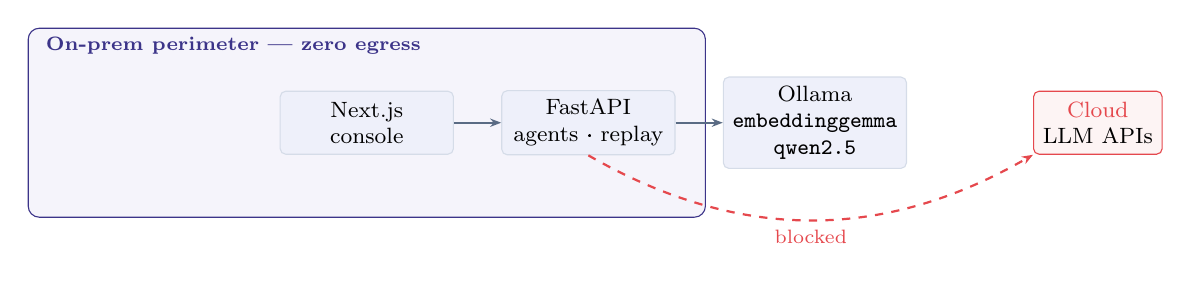
\begin{tikzpicture}[font=\footnotesize,node distance=6mm,
   comp/.style={draw=line,fill=chip,rounded corners=2pt,minimum height=8mm,minimum width=22mm,align=center}]
  \begin{scope}[on background layer]
    \node[draw=violetd,fill=violet!6,rounded corners=4pt,minimum width=8.6cm,minimum height=2.4cm] (peri) {};
  \end{scope}
  \node[anchor=north west,font=\scriptsize\bfseries\color{violetd}] at (peri.north west) {\ On-prem perimeter — zero egress};
  \node[comp] (web) {Next.js\\console};
  \node[comp,right=of web] (api) {FastAPI\\agents · replay};
  \node[comp,right=of api] (oll) {Ollama\\\texttt{embeddinggemma}\\\texttt{qwen2.5}};
  \draw[-{Stealth[length=4pt]},haze,thick] (web)--(api);
  \draw[-{Stealth[length=4pt]},haze,thick] (api)--(oll);
  \node[draw=red,fill=red!6,rounded corners=2pt,right=16mm of oll,align=center,minimum height=8mm] (cloud) {\color{red}Cloud\\LLM APIs};
  \draw[-{Stealth[length=4pt]},red,dashed,thick] (api.south) to[bend right=30] node[below,font=\scriptsize\color{red}]{blocked} (cloud.south west);
\end{tikzpicture}
\end{center}

Classified OT/IT telemetry cannot legally leave the perimeter, so Prahari runs entirely
locally. \texttt{docker-compose} brings up the API, the web console and Ollama; a
\texttt{SOVEREIGN\_MODE} posture enforces zero egress. This is the capability no cloud-API SOC
can offer on national infrastructure — and, as the attribution benchmark showed, cloud models
(\texttt{qwen3.5:cloud}, 397B) returned \texttt{403 Forbidden} without account sign-in, so the
local path is both the fallback and the stronger story.

%============================================================== 9. EVIDENCE ====
\section{Evidence — Measured and Reproducible}

Every claim below is recorded in the repository's \texttt{docs/benchmarks/} and reproducible
from the listed command.

\subsection{Behavioural vs.\ signature on real LANL red-team data}

\begin{center}
\begin{tabularx}{\linewidth}{@{}L{4.2cm} c c c c@{}}
\toprule
\textbf{Detector} & \textbf{Recall} & \textbf{Precision} & \textbf{FPR} & \textbf{TP / FP / FN} \\
\midrule
\textbf{Sentinel} (behavioural) & \textbf{0.794} & 0.004 & 0.075 & 54 / 14{,}941 / 14 \\
Signature (IOC)                 & 0.000 & 0.000 & 0.000 & 0 / 0 / 68 \\
\bottomrule
\end{tabularx}
\end{center}
{\small Window $t\in[759600,770400)$ (densest red-team burst); chronological 50/50 split;
threshold at quantile 0.99. The signature baseline is structurally blind to valid-credential
logins to internal hosts.\par}

\subsection{Cross-source fusion on the red-team host set}

\begin{center}
\begin{tabularx}{\linewidth}{@{}Y c@{}}
\toprule
\textbf{Measure} & \textbf{Result} \\
\midrule
Incidents formed & 102 \\
High-confidence incidents & 21 \\
\ \ …\ of which on red-team hosts & 9 \\
Red-team hosts fused (auth+proc+flow, 3 phases) & \textbf{9 of 11} \\
\bottomrule
\end{tabularx}
\end{center}
{\small Window $t\in[150000,160000)$, correlate by target host, 600\,s window. Compound score
0.80 on each fused red-team incident.\par}

\subsection{Summary scorecard}

\begin{center}
\begin{tabularx}{\linewidth}{@{}Y L{3.4cm} L{4.6cm}@{}}
\toprule
\textbf{Claim} & \textbf{Result} & \textbf{Source} \\
\midrule
Behavioural vs.\ signature recall (real LANL) & \textbf{0.79 vs 0.00} & \texttt{lanl-real-results.md} \\
Real multi-source fusion & 9/11 red-team hosts & \texttt{lanl-multisource-results.md} \\
Air-gapped grounded attribution & C553 → T1021.006 / T1057 / T1071.002 & \texttt{attribution-demo.md} \\
Mean time to detect & weeks → $\approx$seconds (replay) & dashboard \\
Auditability & every incident carries raw evidence & \texttt{CanonicalEvent.raw} \\
\bottomrule
\end{tabularx}
\end{center}

\begin{warnbox}
\textbf{We report the limits honestly.} The fusion benchmark pre-slices to the red-team host
set, so it demonstrates that fusion \emph{is real and forms on genuine APT hosts} — it does not
yet claim precision-at-scale against the full benign population. That requires per-source
anomaly models on process and flow (only auth has a behavioural model today) so that fusion
combines \emph{anomalous} signals rather than raw activity. That is the honest next lift, and it
is scoped in the roadmap.
\end{warnbox}

%============================================================== 10. STACK ======
\section{Implementation}

\subsection{Tech stack}

\begin{center}
\begin{tabularx}{\linewidth}{@{}L{3.6cm} Y@{}}
\toprule
\textbf{Layer} & \textbf{Choice} \\
\midrule
Ingestion / replay & Python generators + timer ($\approx$100$\times$), no Kafka \\
Detection          & scikit-learn Isolation Forest + learned novelty (UEBA); StandardScaler for network \\
Attribution        & Ollama (\texttt{embeddinggemma} + \texttt{qwen2.5:7b}) + numpy cosine retrieval \\
Correlation        & Kill-chain tagging + compound scoring (pure Python) \\
Backend            & FastAPI + Pydantic (async event loop; blocking LLM work off-loaded via \texttt{asyncio.to\_thread}) \\
Frontend           & Next.js 15 (App Router) + React 19 + TypeScript; live SSE + polling; light/dark theming \\
Collectors         & Stdlib Python agents for Linux (\texttt{/proc}, journal) and Windows (Security 4624/4625, Sysmon 1/3) \\
Deploy             & \texttt{docker-compose} · \texttt{SOVEREIGN\_MODE} (zero egress) \\
\bottomrule
\end{tabularx}
\end{center}

\subsection{At a glance}

\begin{center}
\begin{tabularx}{\linewidth}{@{}Y Y Y Y@{}}
\toprule
\textbf{Backend} & \textbf{Frontend} & \textbf{REST endpoints} & \textbf{Tests} \\
\midrule
$\approx$7{,}000 lines Python & $\approx$3{,}400 lines TS/TSX & 30+ \texttt{/api} routes & 50+ test files \\
\bottomrule
\end{tabularx}
\end{center}

\subsection{The SOC console}

The Next.js console is a live operator surface, not a static report:

\begin{itemize}[leftmargin=1.4em,itemsep=2pt]
  \item \textbf{Command view} — an interactive, pan/zoom/replayable attack graph: the focus
        host, lateral-movement peers, public C2 endpoints, and the predicted next node.
  \item \textbf{Incident workspace} — a decision-queue with a ``why this incident'' evidence
        rail (raw records), the ATT\&CK\ attribution panel with per-technique reasoning, and the
        gated response controls.
  \item \textbf{Live telemetry} — fleet health, an event tape with clickable IP enrichment, and
        a live-updating visual summary (stat tiles, donut by type, bars).
  \item \textbf{Settings} — provider selection (Ollama local / Ollama Cloud / OpenAI-compatible),
        model selection, blocklist management, and a light/dark theme toggle.
  \item \textbf{Report} — an AI situation summary with charts and an export path.
\end{itemize}

\subsection{Threat intelligence — fresh, not stale, without full egress}

Threat intel runs offline-first (bundled CIDR blocklist, provider and geo lookups) but can
\emph{optionally} refresh from configurable feed URLs and enrich individual IPs on demand, so
local intelligence does not go stale. Operators can also set their own blocklist entries. The
posture is a deliberate middle ground: air-gapped by default, with explicit, operator-controlled
fetch points — never a silent, always-on egress.

%============================================================== 11. ROADMAP ====
\section{Limitations and Roadmap}

\begin{center}
\begin{tabularx}{\linewidth}{@{}L{5.2cm} Y@{}}
\toprule
\textbf{Known limitation (today)} & \textbf{Planned lift} \\
\midrule
Only auth has a behavioural model; proc/flow fusion uses raw activity & Per-host process baselines + full flow anomaly scoring, so fusion combines \emph{flagged} signals → precision-at-scale \\
Fusion benchmark pre-slices to red-team hosts & Whole-population run separating red-team from benign hosts \\
Digital-twin / vuln agents are lightweight & Full attack-path graph + CVE-driven prioritisation \\
Single-node replay demo & Distributed ingestion for production telemetry volumes \\
\bottomrule
\end{tabularx}
\end{center}

%============================================================== 12. CLOSE ======
\section{Why Prahari Wins}

\begin{keybox}
\begin{enumerate}[leftmargin=1.5em,itemsep=3pt]
  \item \textbf{It detects what signatures cannot} — 79\% recall on real red-team lateral
        movement where IOC detection scores 0\%.
  \item \textbf{The fusion is real, on real data} — the three-sensor ``money moment'' forms on
        9 of 11 genuine LANL red-team hosts, not on synthetic examples.
  \item \textbf{The AI is grounded and honest} — ML detects, the LLM only names attacks from a
        retrieved set behind a hallucination guard; every decision traces to raw evidence.
  \item \textbf{It is sovereign by construction} — fully air-gapped, the one thing a cloud-API
        SOC can never be on classified national infrastructure.
  \item \textbf{We measured, and we report the limits} — every headline number is reproducible,
        and the honest next lift is scoped rather than hidden.
\end{enumerate}
\end{keybox}

%============================================================== APPENDIX =======
\appendix
\section{Appendix — Run It Yourself}

\begin{lstlisting}[language=bash]
# 1. Full stack (API + web + Ollama)
docker-compose up

# 2. API tests
cd apps/api && uv run pytest -v

# 3. Local LLM attribution (air-gapped)
curl -fsSL https://ollama.com/install.sh | sh
ollama pull qwen2.5:7b        # reasoning - writes the explanation
ollama pull embeddinggemma    # embeddings - powers ATT&CK retrieval
ollama serve
#   OLLAMA_HOST=http://localhost:11434
#   PRAHARI_CHAT_MODEL=qwen2.5:7b   PRAHARI_EMBED_MODEL=embeddinggemma

# 4. Reproduce the headline benchmarks
cd apps/api
PYTHONPATH=. uv run python scripts/run_real_benchmark.py 759600 770400 400000
PYTHONPATH=. uv run python scripts/run_multisource_incident.py 150000 160000
PYTHONPATH=. uv run python scripts/run_attribution_demo.py
\end{lstlisting}

\subsection{Selected REST surface}

\begin{center}
\begin{tabularx}{\linewidth}{@{}L{5.4cm} Y@{}}
\toprule
\textbf{Endpoint} & \textbf{Purpose} \\
\midrule
\texttt{GET /api/status} · \texttt{/summary} & Live pipeline + fleet health \\
\texttt{GET /api/events/incidents} & Fused incidents \\
\texttt{GET /api/incidents/\{id\}} & Incident detail + attribution \\
\texttt{GET /api/stream} & SSE live event stream \\
\texttt{GET /api/network/\{ip\}} & IP enrichment (provider · geo · reputation) \\
\texttt{GET/PUT /api/settings} & Provider / model / theme settings \\
\texttt{POST /api/threatintel/refresh} & Optional feed refresh \\
\texttt{GET/POST /api/actions/*} & Response queue + triple gate \\
\bottomrule
\end{tabularx}
\end{center}

\vspace{0.6cm}
\begin{center}
\color{haze}\small Repository: \url{\RepoURL} \quad·\quad Contact: \href{mailto:\ContactEmail}{\ContactEmail}
\end{center}

\end{document}
